% AY2015 制御工学 解答例
% 回答の流れ・言葉遣いは 03_制御工学/参考/「制御工学Ⅱ（完成版）」に寄せる。
% デザイン（囲み枠等）は真似しない。解答・数値は本年度過去問から自力で導いた。
\documentclass[11pt,a4paper]{article}
\usepackage{../../../00_common/preamble}

\usetikzlibrary{positioning,arrows.meta,calc}
\usepackage{pgfplots}
\pgfplotsset{compat=newest}

\title{制御工学 AY2015 解答例（専門応用科目I）}
\author{}
\date{}

\begin{document}
\maketitle

% ==================================================================
\section*{第1問〔I〕}

二次振動系（質量 $m$、粘性係数 $d$、バネ定数 $k$）。

\subsection*{(1) 運動方程式と伝達関数}
質量に働く力のつり合いより
\begin{align*}
  &\qquad m\ddot{x}+d\dot{x}+kx=f(t)\\
  &\therefore\quad (ms^2+ds+k)X(s)=F(s)
   \quad\therefore\quad G(s)=\frac{1}{ms^2+ds+k}.
\end{align*}
\[
  \therefore\quad \ans{\;m\ddot{x}+d\dot{x}+kx=f(t),\qquad G(s)=\dfrac{1}{ms^2+ds+k}\;}
\]

\subsection*{(2) $d,k$ と定常値（$m=1,\ \omega_n=1,\ \zeta=0.5$）}
標準形より $\omega_n^2=\dfrac{k}{m}$、$2\zeta\omega_n=\dfrac{d}{m}$ なので
\begin{align*}
  &\qquad k=m\omega_n^2=1,\qquad d=2\zeta\omega_n m=2\cdot0.5\cdot1=1.
\end{align*}
単位ステップ入力に対する定常値は、安定系では初期値によらず最終値の定理より
$x(\infty)=\lim_{s\to0}\dfrac{1}{s^2+s+1}=1$。
\[
  \therefore\quad \ans{\;d=1,\quad k=1,\quad x(\infty)=1\;}
\]

\subsection*{(3) 無減衰自由応答（$m=1,d=0,k=1$、$x(0)=1,\dot x(0)=0$）}
$f=0$ より $\ddot{x}+x=0$。一般解 $x=A\cos t+B\sin t$ に初期条件を入れて
\begin{align*}
  &\qquad x(0)=A=1,\qquad \dot{x}(0)=B=0.
\end{align*}
\[
  \therefore\quad \ans{\;x(t)=\cos t\;}
\]
減衰がないので振幅 $1$ の持続振動となる。

\begin{center}
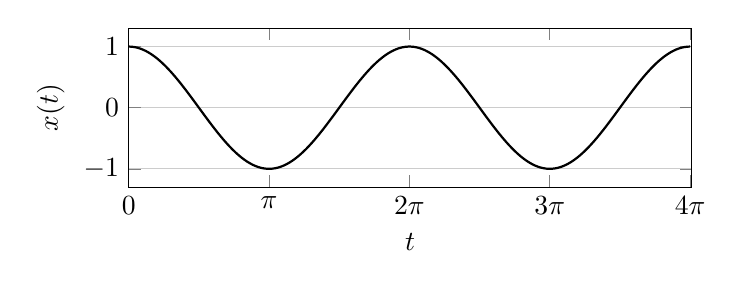
\begin{tikzpicture}
\begin{axis}[
  width=0.72\linewidth, height=3.6cm,
  xmin=0, xmax=12.6, ymin=-1.3, ymax=1.3,
  xlabel={$t$}, ylabel={$x(t)$},
  xtick={0,3.1416,6.2832,9.4248,12.566},
  xticklabels={$0$,$\pi$,$2\pi$,$3\pi$,$4\pi$},
  ytick={-1,0,1}, ymajorgrids=true, grid style={gray!40},
]
\addplot[thick,domain=0:12.566,samples=200]{cos(deg(x))};
\end{axis}
\end{tikzpicture}
\end{center}

\subsection*{(4) 指数入力応答（同パラメータ、$f(t)=\e^{-t}$、$x(0)=1,\dot x(0)=0$）}
$\ddot{x}+x=\e^{-t}$。特解を $x_p=C\e^{-t}$ とおくと $\ddot{x}_p+x_p=2C\e^{-t}=\e^{-t}$ より $C=\tfrac12$。
よって $x=\tfrac12\e^{-t}+A\cos t+B\sin t$。初期条件より
\begin{align*}
  &\qquad x(0)=\tfrac12+A=1,\qquad \dot{x}(0)=-\tfrac12+B=0
   \quad\therefore\quad A=\tfrac12,\ B=\tfrac12.
\end{align*}
\[
  \therefore\quad \ans{\;x(t)=\tfrac12\e^{-t}+\tfrac12\cos t+\tfrac12\sin t\;}
\]
充分な時間が経つと $\e^{-t}\to0$ で、定常項は
$\tfrac12(\cos t+\sin t)=\dfrac{\sqrt2}{2}\sin\!\bigl(t+\tfrac{\pi}{4}\bigr)$ となる。よって振幅の最大値は
\[
  \therefore\quad \ans{\;|x(t)|_{\max}=\dfrac{\sqrt2}{2}\approx0.71\;}
\]
（(3) の振幅 $1$ より減少しており、制御の狙いどおり振幅が抑えられている。）

\bigskip
\noindent 検算: (3)(4) とも導いた $x(t)$ が各微分方程式と初期条件を満たすことを SymPy で確認。
(4) の定常項振幅 $\tfrac12\sqrt{1^2+1^2}=\tfrac{\sqrt2}{2}$✓。

\newpage
% ==================================================================
\section*{第2問〔II〕}

\subsection*{(1) $G_2(s)$ のゲインと位相}
$G_1(s)=\dfrac{1}{20s^2+22s+2}$、$K_0=2$ を直列結合して
\begin{align*}
  &\qquad G_2(s)=\frac{2}{20s^2+22s+2}=\frac{1}{10s^2+11s+1}=\frac{1}{(10s+1)(s+1)}.
\end{align*}
$s=j\omega$ として
\[
  \therefore\quad \ans{\;|G_2(j\omega)|=\dfrac{1}{\sqrt{1+(10\omega)^2}\,\sqrt{1+\omega^2}},\quad
  \angle G_2(j\omega)=-\tan^{-1}10\omega-\tan^{-1}\omega\;}
\]

\subsection*{(2) ゲイン線図（漸近線）}
$|G_2(0)|=1=0\,\mathrm{dB}$。折れ点は $10s+1$ より $\omega=0.1$、$s+1$ より $\omega=1\,[\mathrm{rad/s}]$。
傾きは $\omega<0.1$ で $0$、$0.1<\omega<1$ で $-20$、$\omega>1$ で $-40\,[\mathrm{dB/dec}]$。

\begin{center}
\begin{tikzpicture}
\begin{axis}[
  width=0.86\linewidth, height=5.2cm,
  xmin=1e-2, xmax=1e2, ymin=-100, ymax=20, xmode=log,
  xlabel={$\omega\,[\mathrm{rad/s}]$}, ylabel={ゲイン [dB]},
  ytick={-100,-80,-60,-40,-20,0,20},
  xmajorgrids=true, ymajorgrids=true, xminorgrids=true,
  grid style={line width=0.3pt, draw=gray!60},
  extra y ticks={0}, extra y tick style={grid=major, grid style={line width=1pt, draw=black}},
  legend pos=south west, clip=true, enlargelimits=false,
]
\addplot[thick] coordinates {(0.01,0) (0.1,0) (1,-20) (100,-100)};
\addlegendentry{漸近線}
\addplot[thick,dashed] coordinates
  {(0.01,0.0) (0.1,-3.0) (0.316,-13.2) (1,-23.0) (10,-60.1) (100,-100)};
\addlegendentry{真値}
\node[anchor=south] at (axis cs:0.1,0) {\scriptsize $\omega=0.1$};
\node[anchor=north east] at (axis cs:1,-20) {\scriptsize $\omega=1$};
\end{axis}
\end{tikzpicture}
\end{center}

\subsection*{(3) 単位ステップ応答}
極は実数 $s=-0.1,-1$（過減衰）。$X(s)=\dfrac{G_2(s)}{s}$ を部分分数分解して
\begin{align*}
  &\qquad X(s)=\frac{1}{s(10s+1)(s+1)}
   =\frac{1}{s}-\frac{10/9}{s+0.1}+\frac{1/9}{s+1}\\
  &\therefore\quad x(t)=1-\frac{10}{9}\e^{-0.1t}+\frac{1}{9}\e^{-t}.
\end{align*}
オーバーシュートなく単調に立ち上がり、定常値 $1$ に収束する。整定は遅い極 $s=-0.1$
（時定数 $10\,$s）が支配する。
\[
  \therefore\quad \ans{\;x(t)=1-\dfrac{10}{9}\e^{-0.1t}+\dfrac{1}{9}\e^{-t}\;}
\]

\begin{center}
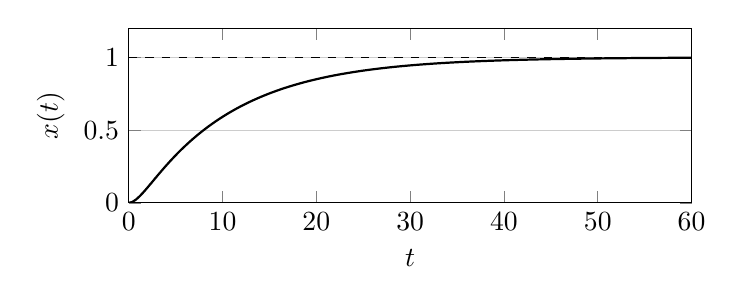
\begin{tikzpicture}
\begin{axis}[
  width=0.72\linewidth, height=3.8cm,
  xmin=0, xmax=60, ymin=0, ymax=1.2,
  xlabel={$t$}, ylabel={$x(t)$},
  ytick={0,0.5,1}, ymajorgrids=true, grid style={gray!40},
]
\addplot[thick,domain=0:60,samples=150]{1-(10/9)*exp(-0.1*x)+(1/9)*exp(-x)};
\addplot[dashed,domain=0:60]{1};
\end{axis}
\end{tikzpicture}
\end{center}

\subsection*{(4) フィードバック系の $K_1$ と過渡特性の比較}
前向き $G_2$、帰還 $G_3(s)=s+1$（出力 $K_1$ の前段で分岐）。閉ループは
\begin{align*}
  &\qquad T(s)=\frac{K_1 G_2}{1+G_2 G_3},\qquad
   G_2G_3=\frac{s+1}{(10s+1)(s+1)}=\frac{1}{10s+1}\\
  &\therefore\quad 1+G_2G_3=\frac{10s+2}{10s+1}\\
  &\therefore\quad T(s)=\frac{K_1}{(10s+1)(s+1)}\cdot\frac{10s+1}{10s+2}
   =\frac{K_1}{2(s+1)(5s+1)}.
\end{align*}
定常値 $T(0)=\dfrac{K_1}{2}$ を (3) の定常値 $1$ に等しくおくと
\[
  \frac{K_1}{2}=1\quad\therefore\quad \ans{\;K_1=2\;}
\]
このとき $T(s)=\dfrac{1}{(s+1)(5s+1)}$、極は $s=-1,\ -0.2$。
\[
  \therefore\quad \ans{\;\text{支配時定数が }G_2\text{ の }10\,\mathrm{s}\ (\text{極}-0.1)\ \to\ 5\,\mathrm{s}\ (\text{極}-0.2)\ \text{に半減}\;}
\]
定常値は $1$ で不変のまま、支配極が $-0.1\to-0.2$ へ移って時定数が半分になり、整定時間も
おおよそ半分に短縮される。依然として実根のみ（過減衰）でオーバーシュートは生じない。
すなわち本フィードバックは定常特性を保ったまま過渡応答を高速化している。

\bigskip
\noindent 検算: $G_2=1/((10s+1)(s+1))$、(3) のステップ応答は $x(0)=0,x(\infty)=1$ で単調増加。
(4) は $T=K_1/(2(s+1)(5s+1))$、$K_1=2$ で極 $\{-1,-0.2\}$ を SymPy で確認✓。

\end{document}
